%%
%% 研究報告用スイッチ
%% [techrep]
%%
%% 欧文表記無しのスイッチ(etitle,eabstractは任意)
%% [noauthor]
%%

\documentclass[techrep,submit,noauthor,platex,dvipdfmx]{ipsj}

% フォントと日本語関連パッケージ
% \usepackage[deluxe,uplatex]{otf}
% \usepackage[T1]{fontenc}

% グラフィックス関連
\usepackage[dvipdfmx]{graphicx} 
\usepackage{subcaption}

% 数式関連
\usepackage{latexsym}
\usepackage{amsmath}
\usepackage{amstext}
\usepackage{amssymb}
\usepackage{multirow}

% その他のパッケージ
\usepackage{url}
\makeatletter
\def\@footyear{2025}
\makeatother

% hyperrefは最後に読み込む
% \usepackage[dvipdfmx,setpagesize=false]{hyperref}

% \def\Underline{\setbox0\hbox\bgroup\let\\\endUnderline}
% \def\endUnderline{\vphantom{y}\egroup\smash{\underline{\box0}}\\}
% \def\|{\verb|}

% \setcounter{巻数}{59}
% \setcounter{号数}{1}
% \setcounter{page}{1}


% \受付{2016}{3}{4}
% \再受付{2015}{7}{16}   %省略可能
% \再再受付{2015}{7}{20} %省略可能
% \再再受付{2015}{11}{20} %省略可能
% \採録{2016}{8}{1}




\begin{document}


\title{Nタプルネットワークの大きさと学習性能の関係:\\ミニ2048を用いた実験・評価}

% \etitle{}

% \affiliate{IPSJ}{情報処理学会\\
% IPSJ, Chiyoda, Tokyo 101--0062, Japan}


\affiliate{KUTGE}{高知工科大学大学院工学研究科}
\affiliate{KUTSI}{高知工科大学情報学群}

% \paffiliate{JU}{高知工科大学\\
% Kochi University of Technology\\}

\author{寺内 俊輔}{Shunsuke Terauchi}{KUTGE}[295141a@gs.kochi-tech.ac.jp]
\author{松崎 公紀}{Kimnori Matsuzaki}{KUTSI}[matsuzaki.kiminori@kochi-tech.ac.jp]

\begin{abstract}
    2048では、NタプルネットワークとTD学習を拡張した手法及びExpectimax探索の組み合わせにより優れたプレイヤが作られている.
    本研究では、ミニ2048において構築可能な1タプルから9タプルまでの各タプル全てからなる組み合わせと、それぞれにおける妥当な形状を用いて、Nタプルネットワークの大きさと学習性能の関係を実験的に評価する.
    特に最先端プレイヤの開発で用いられた手法の観点から、その効果と特性について考察を行う.
\end{abstract}

\begin{jkeyword}
2048, Nタプルネットワーク, Expectimax探索, ミニ2048, 強化学習
\end{jkeyword}

% \begin{eabstract}
% This document is a guide to prepare a draft for submitting to IPSJ
% Journal, and the final camera-ready manuscript of a paper to appear in
% IPSJ Journal, using {\LaTeX} and special style files.  Since this
% document itself is produced with the style files, it will help you to
% refer its source file which is distributed with the style files.
% \end{eabstract}

% \begin{ekeyword}
% IPSJ Journal, \LaTeX, style files, ``Dos and Don'ts'' list
% \end{ekeyword}
\maketitle
\section{はじめに}
「2048」はG.~Cirulliによって作られた確率的一人ゲームであり~\cite{2048}.
これまでにさまざまなコンピュータプレイヤが作られてきた.
現在最も成功しているアプローチは,強化学習によってチューニングしたNタプルネットワーク評価関数~\cite{SzJa14}とExpectimax探索~\cite{YWHC16}を組み合わせるものである.
その後,NタプルネットワークとExpectimax探索の組合せを基礎として,一般的もしくはゲームに特化した改良手法が多数提案されてきた~\cite{YWHC16,Mats17,Jask17,GuCW22}.
Gueiによって作られた最先端プレイヤ~\cite{GuCW22}では,大きさ6のタプル8個からなるネットワーク2つを切り替えて用いる評価関数,より幅広く学習するためのOptimistic Initialization,ゲーム特化型の改良手法であるTile downgrading,およびExpectimax探索を組み合わせることで,平均得点 625\,377 を達成した.

Nタプルネットワークやニューラルネットワークでは,一般に,ネットワーク内のパラメータ数が増えるほど性能が向上すると言われている~\cite{kaplan2020scaling}.一方で,パラメータ数が増えすぎると,学習に必要となるデータが莫大になるという問題に加えて,過学習(過適合)の問題も発生する.

2048のコンピュータプレイヤにおいては,これまでネットワークのパラメータ数を増やすことで性能向上が図られてきた.
2048にNタプルネットワークを用いる最初の研究である Szubert と Ja\'{s}kowski による研究~\cite{SzJa14}では,まず大きさ4のタプル17個からなるネットワーク(パラメータ数$1.11\times 10^6$)が用いられ,次に6タプル2個と4タプル2個からなるネットワーク(パラメータ数$3.37\times 10^7$)が用いられていた.
続く Wuらによる研究~\cite{WYLC14}では,ネットワークが大きさ6のタプル4つからなるもの(パラメータ数$6.71\times 10^7$)へ拡張された.
2018年時点での最先端プレイヤ~\cite{Jask17}では,6タプル5個にredundant encodingを組み合わせたネットワーク(パラメータ数 $8.42\times 10^7$)16個をゲーム進行に合わせて切り替える手法がとられている.論文投稿時点のGuei による最先端プレイヤ~\cite{GuCW22}では,Matsuzak~\cite{Mats16}が実験的に求めた6タプル8つの組合せ(パラメータ数 $1.34\times 10^8$)2つを切り替えて用いている.このGuei によるプレイヤの学習では,Optimistic Initialization を用いてより幅広く学習する工夫が取り入れられている.
一方,ニューラルネットワークによる評価関数を用いるプレイヤでは,Matsuzaki~\cite{Mats19}が,畳み込みネットワークのパラメータ数を $1.85\times 10^5$ から $2.90\times 10^6$ まで変化させたときに性能が向上することを報告している.

ここで生じる疑問は,2048のNタプル評価関数において,性能向上が見られる範囲でどこまでパラメータ数を増やしていけるのか,という点である.Oka と Matsuzaki~\cite{OkMa16b},および,Matsuzaki~\cite{Mats16} は,大きさ6のタプルだけでなく,大きさ7のタプル複数個を系統的に組み合わせる手法を示し,同一条件での比較においては大きさ6のネットワークよりも大きさ7 のネットワークのほうが性能が高くなりうることを示した.
しかしながら,大きさ8のタプルからなるネットワークでは,単純に実装するとパラメータ数が $4.29\times 10^{12}$ と巨大になり,メモリサイズおよび学習コストの観点から,現時点では実現は困難である.


そこで本研究では,大きさが小さくパラメータ数を減らすことができ,また,すでに完全解析による真の正解が分かってるミニ2048を用いて,NタプルネットワークのタプルサイズとOptimistic Initialization(OI)の初期値がプレイヤの性能に与える影響について実験的に評価する.本研究の実施にあたって設定したリサーチクエスチョンは次の3つである.
\begin{itemize}
\item \textbf{RQ1} Nタプルネットワークにおけるタプルの大きさ,数,パラメータ数に対して,スコアにどのような影響があるか.
\item \textbf{RQ2} 幅広く強化学習を行う Optimistic Initialization の初期値を変えたときに,Nタプルネットワークの学習にどのような影響があるか.
\item \textbf{RQ3} Nタプルネットワーク評価関数とExpectimax探索とを組み合わせたとき,探索による性能向上はNタプルネットワークとその学習方法に依存するか.
\end{itemize}

本研究では,まず,タプルの大きさを1から9とし,そのそれぞれについて2種類のタプルの組合せによるNタプルネットワークを設計した.設計したNタプルネットワークに対し,Optimistic Initialization の初期値を変えた学習を行い,Expectimax 探索の深さを変えて各プレイヤの平均得点を調べた.これらの網羅的な実験の結果,以下に示す知見が得られた.
\begin{itemize}
\item RQ1に関して,パラメータ数の対数とスコアの間にはおよそ二次関数(放物線)の関係が見られる.とくに,タプルの大きさが 5 から 6 のときに性能のピークがある.
\item RQ2に関して,Optimistic Initializationの初期値が小さすぎる($\mbox{\itshape OI} = 0$)場合には,低いスコアで学習が止まってしまう場合がある.逆に,初期値が大きすぎる($\mbox{\itshape OI} = 5400$)場合には,パラメータ数が多くなると学習が停滞することが見られた.初期値が適切である($\mbox{\itshape OI} = 1200$)場合,学習が安定して進むだけでなく,より多くのパラメータ数からなるネットワークでスコアが最大化する効果が見られた.
\item RQ3に関して,Expectimax探索によるスコアの向上は,Optimistic Initialization の初期値やパラメータ数には大きく影響されない結果となった.具体的には,探索深さ  1(Greedy)から6に増やすと,理想的なq最高平均得点5469点までの距離がおよそ半分に減っていた.
\end{itemize}

% 以上の結果は,2048型ゲームにおけるNタプルネットワークの構成や初期化戦略とプレイヤの性能の関係を解明する重要な一歩である.{\color{red}この文はまとめに移してはどうか?}
\section{ミニ2048}
本研究はミニ2048~\cite{YaKN22J}を研究対象として使用する.
ミニ2048は,$3\times 3$ の盤面でプレイされることを除いて,確率的一人ゲーム{2048}と同じゲームである.

\subsection{ルール}

ミニ2048は,$3\times 3$ の盤面でプレイされる.
初期局面は9マスの内どこか2マスに2(確率0.9)か4(確率0.1)の数字タイルがランダムに置かれた盤面からなる.

各局面において,プレイヤは上下左右いずれかの方向を選択する.
すると各数字タイルはその方向にできるだけ移動する.
移動した結果,2つの同じ数字のタイルが移動方向に衝突するとこれらは合体してその合計値のタイルとなり,
その合計値がスコアに加算される.合体してできたタイルは,同じターンでは別のタイルと合体することはない.
例えば,盤面の行が \verb*|_2_|,\verb*|22_|,\verb*|422| であるとき,右を選択するとそれぞれ \verb*|__2|,\verb*|__4|,\verb*|_44| へと変化する.
その後,空白のマスのうちのランダムな1マスに2(確率0.9)か4(確率0.1)のタイルが置かれる.

プレイヤはいずれかのタイルが移動または衝突するような方向しか選択することができない.いずれの方向も選択できなくなるとゲームは終了する.
このゲームの目標はゲームが終了する前に出来るだけ高得点を獲得することである.

\subsection{用語の導入}
通常の2048と同様にミニ2048における1ターンは,「移動・合体ステップ」と「新規タイルステップ」の2ステップからなる.これらステップの前後の状態を区別するため,以下の用語を導入する.
\begin{figure}[t]
  \centering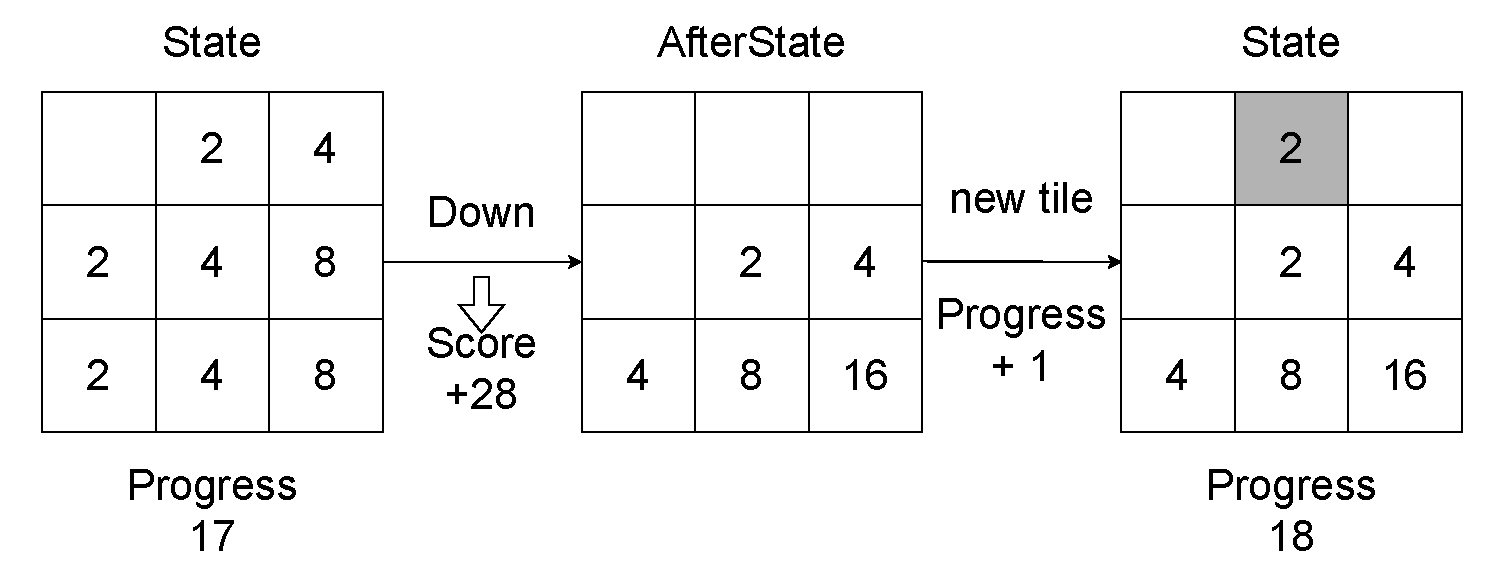
\includegraphics[width=.99\linewidth]{pdf/state_afterstate.drawio.pdf}
  \caption{state,afterstate,progressの例}
  \label{afterstate}
 \end{figure}
\begin{description}
  \item[state] プレイヤが手を選択する盤面状態(とスコア)を\emph{state}と呼ぶ.
  \item[afterstate] プレイヤが手を選択してタイルが移動・合体した直後の盤面状態(とスコア)を\emph{afterstate}と呼ぶ.すなわち,afterstateは新規タイルが出現する前の盤面状態である.
 \end{description}

(通常の2048同様に)ミニ2048では,新しく出現するタイルはランダムに 2 か 4 の値をとる.そのため,単純にターン数をゲームの流さや進行度の指標に用いるには不都合がある.
この問題を解決するため,本研究では以下の指標を用いる.
\begin{description}
  % (\emph{時刻}~\cite{YaKa23J})これ抜いた
 \item[progress] タイルの値の合計値の半分を\emph{progress}~\cite{TeKM23}と呼ぶ.progress は,1ターンで1(新規タイルが2の場合)または2(新規タイルが4の場合)だけ増加する.
\end{description}

図\ref{afterstate}は,初期局面から始まるゲームの流れにおいて,state,afterstate,progress について図示したものである.


\subsection{完全解析とその結果}

ミニ2048は確率的一人ゲームであり,その完全解析とは各状態に対して期待スコア求めることである.
ミニ2048は,到達可能な状態数が $10^9$ 以下と小さいため,現実的な時間で完全解析ができる.
山下ら~\cite{YaKN22J}は,ミニ2048の完全解析に最初に取り組み,そこでは幅優先探索による状態列挙と,列挙した状態を用いる後退解析を行った.
また,著者ら~\cite{TeKM23}も完全解析の追試を行い,深さ優先探索による後退解析で,結果の正しさを確認した.

完全解析の結果について,重要なものを以下に示す.
初期状態のいずれかから到達可能な state の数は 48\,713\,519,afterstate の数は 31\,431\,374 である.
初期状態の期待スコアは,5\,468.49 である.
各 afterstate に対する期待スコアを格納したものを valueDB と呼ぶ.

完全解析で得られる valueDB を用いると,各局面において最適な手を選択するパーフェクトプレイヤを実現できる.
ただし,ミニ2048は確率的一人ゲームのため,決定的に最善手を選択するパーフェクトプレイヤであっても,ゲームごとに
プレイの結果は異なることに注意が必要である.
図\ref{pp-play}は,パーフェクトプレイヤが1万ゲームを行った際の,progress ごとの生存率とゲーム終了時のスコアを示している.
表\ref{pp-specific}は,パーフェクトプレイヤが256,512,1024タイルに到達したときの進捗状況,スコア,生存率を示している.
パーフェクトプレイヤでも,512タイルに到達した後,1024タイルに到達する前は,生存率が急激に低下することが分かる.
図\ref{pp-play}より,生存率が急激に下がるタイミングがいくつかある.
本研究では,そのような生存率が下がる部分を\emph{難易度の高い領域}と呼ぶ.
\begin{table}[t]
  \caption{Progress, score, and alive ratio of perfect player}
  \label{pp-specific}
  \centering\begin{tabular}{lrrr}
   \hline\hline
   Condition & ~~Progress & ~~~~Score~ & ~~~~~~Alive~~ \\
   \hline
  256-tile                          & 136~~~ & 1\,750~ & 99.53\% \\
  512-tile                          & 263~~~ & 4\,000~ & 73.84\% \\
  512-tile \& 256-tile              & 391~~~ & 5\,750~ & 54.40\% \\
  512-tile \& 256-tile \& 128-tile  & 456~~~ & 6\,500~ & 40.49\% \\
  1024-tile                         & 511~~~ & 9\,000~ &  1.07\% \\
   \hline
\end{tabular}
\end{table}

\begin{figure}[t]
  \centering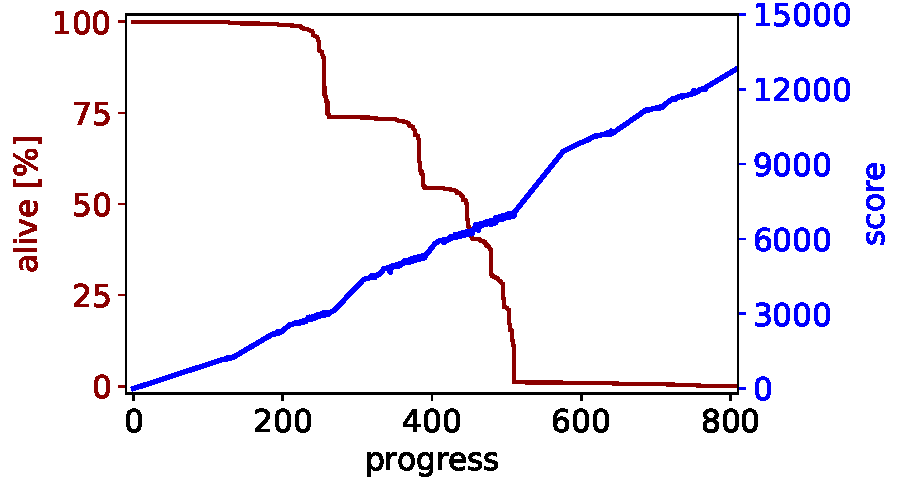
\includegraphics[width=\linewidth]{pdf/pp-play.pdf}
  \caption{パーフェクトプレイヤの生存率とスコア \cite{TeKM23}}
  \label{pp-play}
\end{figure}

% \section{パーフェクトプレイヤの結果を用いたミニ2048の分析}
% \subsection{プレイヤにノイズを加えた場合の平均得点の変化}

% 一般に,stateやafter stateの評価関数は完全に正確であるとは限らない.そこ,で評価関数が不正確な場合のスコアの変化を調査するため,valueDB にノイズを加えたシミュレーションを行った.
% ノイズは平均 0,分散 $\sigma^2$ の正規分布から生成し,標準偏差 $\sigma$ を 0 から 500 まで変化させた.
% このように変化させた valueDB を用いる貪欲プレイヤに 10,000 回のゲームをプレイさせ,その平均スコアを図~\ref{error_averagescore} に示す.

% % \begin{figure} 
% %   \centering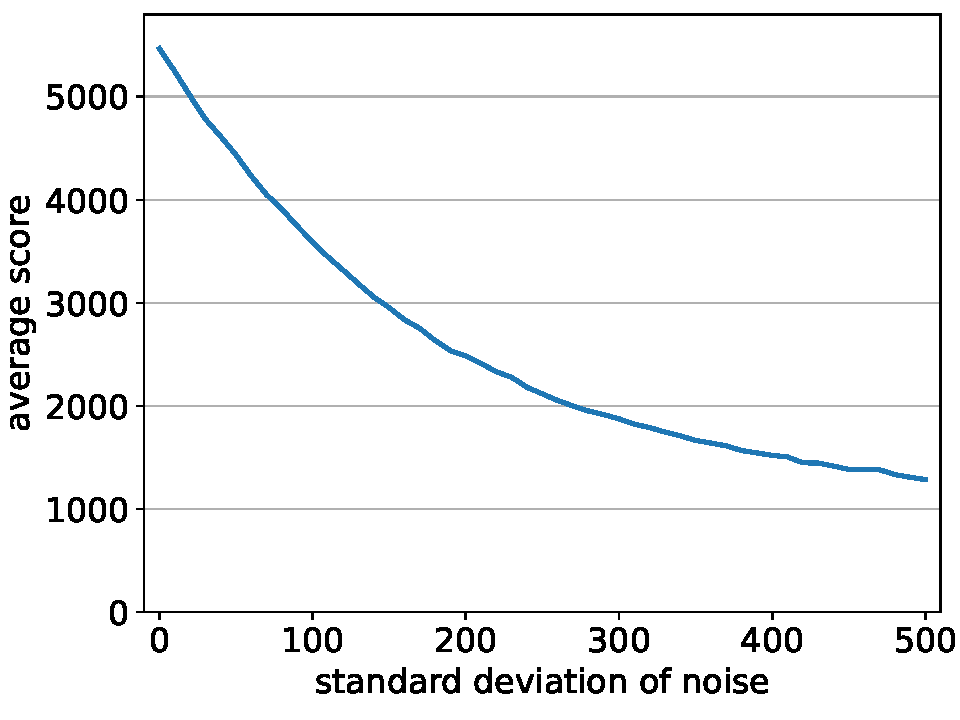
\includegraphics[height=0.40\textheight]{pdf/error_averagescore.pdf} 
% %   \caption{ノイズを加えたプレイヤの平均スコア} 
% %   \label{error_averagescore} 
% % \end{figure}

% 図~\ref{error_averagescore} より,標準偏差 $\sigma$ を大きくすると,平均スコアは単調に減少することが確認できる.
% 例えば,平均スコアが 5000,4000,3000,2000 となる $\sigma$ の値は,それぞれ $\sigma \approx 25, 75, 145, 270$ であった.

\section{本研究で用いるプレイヤ}
\subsection{Nタプルネットワーク評価関数}
\label{sec:Ntuple}

2048における最も成功したプレイヤの多くは、Nタプルネットワークに基づく評価関数を強化学習によってチューニングするアプローチを採用している~\cite{SzJa14}。
Gueiらの最新のプレイヤ~\cite{GuCW22}も、Matsuzaki~\cite{Mats16}が提案したタプルの組合せをベースに、Expectimax探索やMultistaging\cite{YWHC16}、Optimistic Initialization、Tile Downgrading\cite{GuCW22}などの改良を加えることで高い性能を達成している。

本研究では、こうした知見を踏まえ、ミニ2048において1タプルから9タプルまでのNタプルネットワークを構築可能な全てのタプル列挙を行い、
\begin{itemize}
  \item 我々が妥当と判断した形状のみを選んだタプル集合
  \item 各サイズごとの連続タイルすべてを使用したタプル集合
\end{itemize}
    という2通りの設計方針でネットワークを構築した。

この結果、最大で18種類のNタプルネットワークが得られたが、1タプル、2タプル、9タプルにおいては両方の設計が一致したため、プレイヤの種類としては15通りとなった。
これらのプレイヤを用いて、Nタプルネットワークの大きさ(タプル数)と学習性能の関係を実験的に評価した。

表\ref{tuples}に、本研究で使用したタプルの構造を示す。
また、ミニ2048の盤面の持つ対称性(回転・反転)**を活用し、1つのタプルに対して対称な8通りの位置からのサンプリングを行うことで、学習に必要なタプル数の削減を図っている。

\begin{table}[t]
  \caption{タプルサイズと形状の一覧}
  \label{tuples}
  \centering\begin{tabular}{ll}
   \hline
   \hline
   タプル名 & \hspace{20pt}タプルの形状 \\
   \hline
   \raisebox{10pt}{NT1F}\raisebox{28pt}{~}
          & 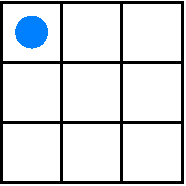
\includegraphics[height=22pt]{pdf/tuples/1tuple_6_page1.pdf}~
            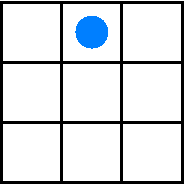
\includegraphics[height=22pt]{pdf/tuples/1tuple_6_page2.pdf}~
            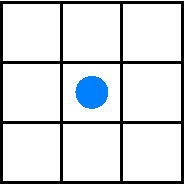
\includegraphics[height=22pt]{pdf/tuples/1tuple_6_page3.pdf}\\
   \hline
   \raisebox{10pt}{NT2F}\raisebox{28pt}{~}
          & 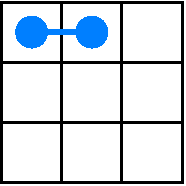
\includegraphics[height=22pt]{pdf/tuples/2tuple_12_page1.pdf}~
            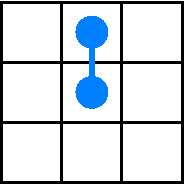
\includegraphics[height=22pt]{pdf/tuples/2tuple_12_page2.pdf}\\
   \hline
   \raisebox{10pt}{NT3M}\raisebox{28pt}{~}
          & 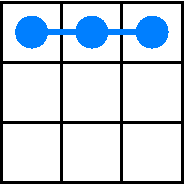
\includegraphics[height=22pt]{pdf/tuples/3tuple_144_page1.pdf}~
            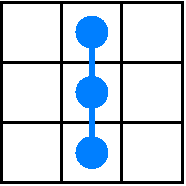
\includegraphics[height=22pt]{pdf/tuples/3tuple_144_page3.pdf}~
            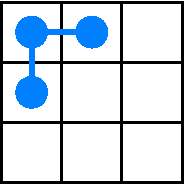
\includegraphics[height=22pt]{pdf/tuples/3tuple_144_page2.pdf}\\
   \hline
   \raisebox{10pt}{NT3F}\raisebox{28pt}{~}
          & 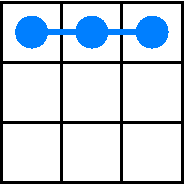
\includegraphics[height=22pt]{pdf/tuples/3tuple_2673_page1.pdf}~
            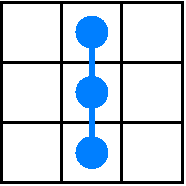
\includegraphics[height=22pt]{pdf/tuples/3tuple_2673_page5.pdf}~
            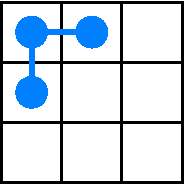
\includegraphics[height=22pt]{pdf/tuples/3tuple_2673_page2.pdf}~
            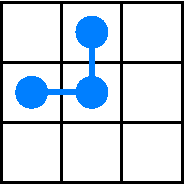
\includegraphics[height=22pt]{pdf/tuples/3tuple_2673_page4.pdf}~
            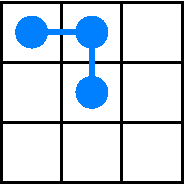
\includegraphics[height=22pt]{pdf/tuples/3tuple_2673_page3.pdf}\\
   \hline
   \raisebox{10pt}{NT4M}\raisebox{28pt}{~}
          & 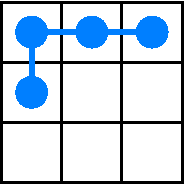
\includegraphics[height=22pt]{pdf/tuples/4tuple_301_page1.pdf}~
            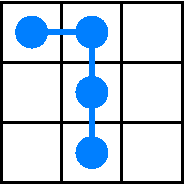
\includegraphics[height=22pt]{pdf/tuples/4tuple_301_page3.pdf}~
            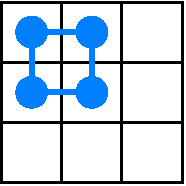
\includegraphics[height=22pt]{pdf/tuples/4tuple_301_page2.pdf}\\
   \hline
   \raisebox{10pt}{NT4F}\raisebox{28pt}{~}
          & 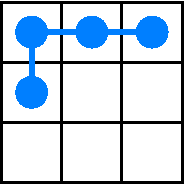
\includegraphics[height=22pt]{pdf/tuples/4tuple_44755_page1.pdf}~
            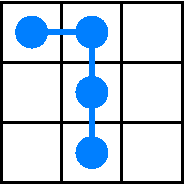
\includegraphics[height=22pt]{pdf/tuples/4tuple_44755_page5.pdf}~
            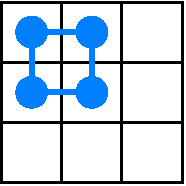
\includegraphics[height=22pt]{pdf/tuples/4tuple_44755_page3.pdf}\\
          & 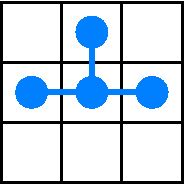
\includegraphics[height=22pt]{pdf/tuples/4tuple_44755_page6.pdf}~
            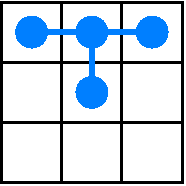
\includegraphics[height=22pt]{pdf/tuples/4tuple_44755_page2.pdf}~
            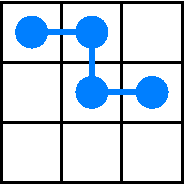
\includegraphics[height=22pt]{pdf/tuples/4tuple_44755_page4.pdf}\\
   \hline
   \raisebox{10pt}{NT5M}\raisebox{28pt}{~}
          & 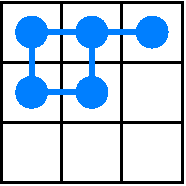
\includegraphics[height=22pt]{pdf/tuples/5tuple_298_page1.pdf}~
            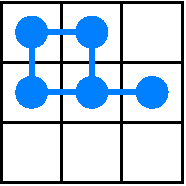
\includegraphics[height=22pt]{pdf/tuples/5tuple_298_page2.pdf}~
            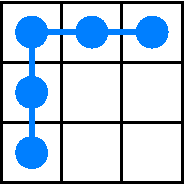
\includegraphics[height=22pt]{pdf/tuples/5tuple_298_page3.pdf}\\
   \hline
   \raisebox{10pt}{NT5F}\raisebox{28pt}{~}
          & 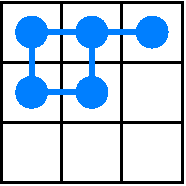
\includegraphics[height=22pt]{pdf/tuples/5tuple_896673_page1.pdf}~
            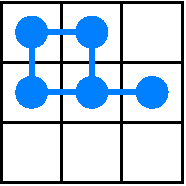
\includegraphics[height=22pt]{pdf/tuples/5tuple_896673_page3.pdf}~
            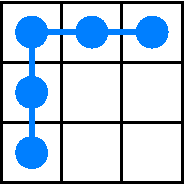
\includegraphics[height=22pt]{pdf/tuples/5tuple_896673_page4.pdf}~
            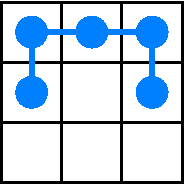
\includegraphics[height=22pt]{pdf/tuples/5tuple_896673_page2.pdf}~
            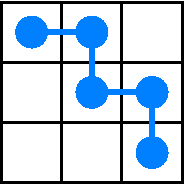
\includegraphics[height=22pt]{pdf/tuples/5tuple_896673_page5.pdf}\\
          & 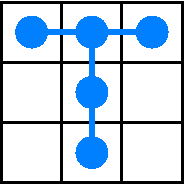
\includegraphics[height=22pt]{pdf/tuples/5tuple_896673_page6.pdf}~
            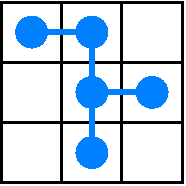
\includegraphics[height=22pt]{pdf/tuples/5tuple_896673_page7.pdf}~
            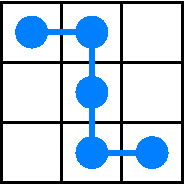
\includegraphics[height=22pt]{pdf/tuples/5tuple_896673_page8.pdf}~
            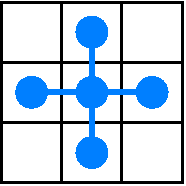
\includegraphics[height=22pt]{pdf/tuples/5tuple_896673_page9.pdf}\\
   \hline
   \raisebox{10pt}{NT6M}\raisebox{28pt}{~}
          & 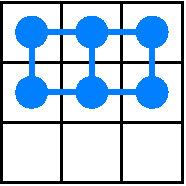
\includegraphics[height=22pt]{pdf/tuples/6tuple_16_page1.pdf}~
            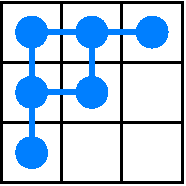
\includegraphics[height=22pt]{pdf/tuples/6tuple_16_page2.pdf}\\
   \hline
   \raisebox{10pt}{NT6F}\raisebox{28pt}{~}
          & 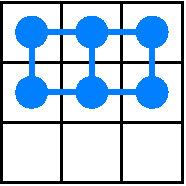
\includegraphics[height=22pt]{pdf/tuples/6tuple_26835_page1.pdf}~
            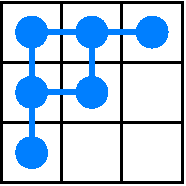
\includegraphics[height=22pt]{pdf/tuples/6tuple_26835_page2.pdf}~
            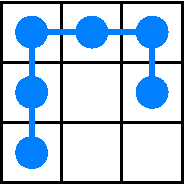
\includegraphics[height=22pt]{pdf/tuples/6tuple_26835_page3.pdf}~
            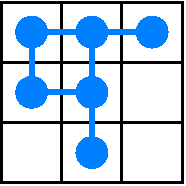
\includegraphics[height=22pt]{pdf/tuples/6tuple_26835_page4.pdf}\\
          & 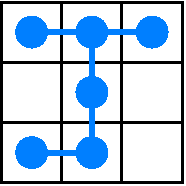
\includegraphics[height=22pt]{pdf/tuples/6tuple_26835_page5.pdf}~
            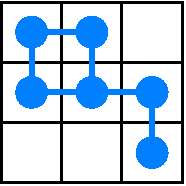
\includegraphics[height=22pt]{pdf/tuples/6tuple_26835_page6.pdf}~
            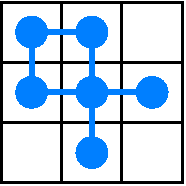
\includegraphics[height=22pt]{pdf/tuples/6tuple_26835_page7.pdf}~
            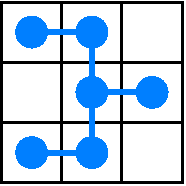
\includegraphics[height=22pt]{pdf/tuples/6tuple_26835_page8.pdf}\\
   \hline
   \raisebox{10pt}{NT7M}\raisebox{28pt}{~}
          & 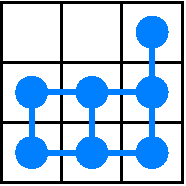
\includegraphics[height=22pt]{pdf/tuples/7tuple_0_page1.pdf}\\
   \hline
   \raisebox{10pt}{NT7F}\raisebox{28pt}{~}
          & 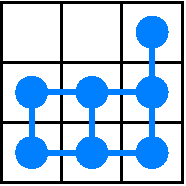
\includegraphics[height=22pt]{pdf/tuples/7tuple_248_page1.pdf}~
            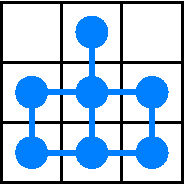
\includegraphics[height=22pt]{pdf/tuples/7tuple_248_page2.pdf}~
            \includegraphics[height=22pt]{pdf/tuples/7tuple_248_page3.pdf}~
            \includegraphics[height=22pt]{pdf/tuples/7tuple_248_page4.pdf}\\
          & \includegraphics[height=22pt]{pdf/tuples/7tuple_248_page5.pdf}~
            \includegraphics[height=22pt]{pdf/tuples/7tuple_248_page6.pdf}~
            \includegraphics[height=22pt]{pdf/tuples/7tuple_248_page7.pdf}\\
   \hline
   \raisebox{10pt}{NT8M}\raisebox{28pt}{~}
          & \includegraphics[height=22pt]{pdf/tuples/8tuple_0_page1.pdf}\\
   \hline
   \raisebox{10pt}{NT8F}\raisebox{28pt}{~}
          & \includegraphics[height=22pt]{pdf/tuples/8tuple_6_page1.pdf}~
            \includegraphics[height=22pt]{pdf/tuples/8tuple_6_page2.pdf}~
            \includegraphics[height=22pt]{pdf/tuples/8tuple_6_page3.pdf}\\
   \hline
   \raisebox{10pt}{NT9F}\raisebox{28pt}{~}
          & \includegraphics[height=22pt]{pdf/tuples/9tuple_0_page1.pdf}\\
   \hline
  \end{tabular}
\end{table}

Nタプルネットワークの重みは,afterstate 間の評価値の差に基づくTD学習法の改良手法によって調整した.
本研究で用いるNタプルネットワークの学習では,以下の技術を用いた.
\begin{description}
  % \item [対称性サンプリング] 各タプルについて,鏡面,回転対称用いてを1つの盤面から,8つの対称位置からサンプリングする. これにより,少ないタプル数で盤面全体から特徴を抽出することができる.
  \item [Multistaging] ゲームの進行に応じて重みを参照するテーブルを切り替える.本研究では,2ステージとし,512 のタイルができる前後でステージを分けた.
  \item [Temporal coherence 学習(TC学習)] TC学習は学習率自動調整機能を備えたTD学習で,Ja\'{s}kowski~\cite{Jask17}が始めて2048に導入した.
  \item [Optimistic initialization] 学習段階での探索を広く行うために,重みを(ゼロではなく)大きな値で初期化する.本研究で用いたNタプルの学習では,すべての afterstate の初期値が 1200 になるように重みを初期化してある.
\end{description}

それぞれのNタプルニューラルネットワークに対して,$5\times 10^8$ 局面分のデータで学習を行った.いずれのニューラルネットワークも,十分に学習が収束していることを確認してある~\cite{TeKM23}.
% \newpage
\section{Expectimax探索}
\label{sec:expectimax}
Expectimax探索は,確率的一人ゲームにおける標準的な探索手法である.
ミニ2048のゲームの進行は,state におけるプレイヤの選択と,afterstate における新規タイルの出現が交互に起こる.
したがって,ミニ2048のゲーム木は,根が現在の state に対応し,根から葉への各パス上に,afterstate に対応するノード(chance ノード)と state に対応するノード(max ノード)が交互に現れる.本研究では,ミニ2048のゲーム木の高さ(探索の深さ)を,各パス上の afterstate に対応するノードの数と定める.例えば,高さ2 のミニ2048のゲーム木は,根,afterstate に対応するノードの層,state に対応するノードの層,afterstate に対応するノードの層,の合計4層からなる(図~\ref{result.Expectimax}).

Expectimax探索では,ゲーム木の各ノードに対して次のように再帰的に計算を行う.
\begin{itemize}
 \item maxノードでは,子要素の値のうちの最大値を計算する.
 \item chanceノードでは,子要素の値を,その出現確率を用いた重み付き平均を計算する.
\end{itemize}
Expectimax探索プレイヤは,Expectimax探索によって得られた子ノードのうち,評価値の最も大きなものを選択する.

図\ref{result.Expectimax}に深さ2のExpectimax探索の例を示す.

\begin{figure}[t]
  \centering
  \includegraphics[width=.99\linewidth]{pdf/expectimax.pdf}
  \caption{深さ 2 のExpectimax 探索の例}
  \label{result.Expectimax} 
\end{figure}

ミニ2048のゲーム木では,特に,同じ afterstate が複数出現する.
そのような同じ afterstate をまとめる(合流)工夫を実装した.ただし,合流を考慮しない Expectimax と結果が一致するよう,同じ afterstate であってもゲーム木中の深さが異なる場合には別のものとして扱った.この工夫により,特に深い探索において大幅な高速化が実現された.
本研究では\cite{Terauchi24}で実装したExpectimax探索を用いた.
% \newpage
\section{実験}

前節で説明した方法により,15種類のNタプルネットワークのそれぞれについて,Optimistic initialization の初期値 $\mathit{OI}$ を3通り変えて学習を行った.
ランダム性の影響を抑えるため,各条件について乱数のシードを変えて10回の学習を行い,10個のNタプルネットワークを得た.
次に,各Nタプルネットワークに対し,GreedyプレイおよびExpectimax探索(深さ2〜6)により1000ゲームのプレイを行い,それらの平均スコアを求めた.
本節のグラフにおいて,10個のNタプルネットワークの平均を点や線で示し,それらの標準偏差をエラーバー等で示す.

% 本研究では,ミニ2048におけるNタプルネットワークの学習性能を多角的に分析するため,
% 構造の異なる複数のプレイヤを構築し,GreedyおよびExpectimax探索による評価を行った.

% \ref{tuples}で示した15種類のプレイヤを用いて評価を行った.

% さらに,Optimistic Initialization(OI)の影響を調べるため,
% 各プレイヤについてOIの初期値を0,1200,5400に設定し,それぞれ学習を実施した.
% すべてのプレイヤは $5 \times 10^8$ 手分の行動に基づいて学習を行い,
% 乱数シードを変えて10体ずつ学習させた.結果として,
% $15$タプル構成$\times 3$回(OIの初期値)$\times 10$回(シード)で,計$450$体のプレイヤが作成された.

% これらのプレイヤに対して,1000ゲームプレイを行い,
% seed違いの結果をまとめた10000ゲームのログを用いて解析を行なった.

\subsection{スコアとパラメータ数の関係}
第1節で示した RQ1 について考察するため,Greedy プレイのスコアを,Optimistic initialization の初期値($\mathit{OI}$)ごとにプロットしたものが図\ref{fig:score_vs_tuple_OI0}から図\ref{fig:score_vs_tuple_OI5400}である.これらのグラフは,横軸にパラメータ数の対数をとり,縦軸にスコアの平均値と標準偏差をプロットしている.また,それぞれのグラフの点に対し,パラメータ数の対数とスコアの関係を二次関数でフィッティングして得られる近似曲線も描いている.

これらのグラフから,いずれのグラフもおよそ放物線を描いていることが分かる.
とくに,\textsf{5M}から\textsf{6F}の区間に放物線の頂点が位置することが確認できた.
また,$\mathit{OI}=0$の場合(図\ref{fig:score_vs_tuple_OI0}),3種類の初期値の中で標準偏差が大きいものが目立っている.このことは,Optimistic initializationを行わない学習では,学習の幅広さが足りず,安定的に良い結果が得られないことを意味する.
$\mathit{OI}=1200$ と $\mathit{OI}=5400$の場合(図\ref{fig:score_vs_tuple_OI1200},図\ref{fig:score_vs_tuple_OI5400}),スコアのばらつきは小さい.
また,より多くのパラメータ数のところまでスコアの向上が見られる(すなわち,放物線の頂点が右に移動する).
\textsf{5F}よりもパラメータ数の少ないNタプルネットワークでは,平均スコアは初期値にそれほど依存していない.一方,それよりも多くのパラメータを持つNタプルネットワークでは,初期値が $\mathit{OI}=1200$ の場合に最も良い結果が得られた.

\begin{figure}[t]
    \centering
    \begin{subfigure}[b]{\linewidth}
        \centering
        \includegraphics[width=\linewidth]{pdf/parameter_performance_plots/params_performance_OI0_EXP1.pdf}
        \caption{OI=0}
        \label{fig:score_vs_tuple_OI0}
    \end{subfigure}

    \vspace{1em}
    \begin{subfigure}[b]{\linewidth}
        \centering
        \includegraphics[width=\linewidth]{pdf/parameter_performance_plots/params_performance_OI1200_EXP1.pdf}
        \caption{OI=1200}
        \label{fig:score_vs_tuple_OI1200}
    \end{subfigure}

    \vspace{1em}
    \begin{subfigure}[b]{\linewidth}
        \centering
        \includegraphics[width=\linewidth]{pdf/parameter_performance_plots/params_performance_OI5400_EXP1.pdf}
        \caption{OI=5400}
        \label{fig:score_vs_tuple_OI5400}
    \end{subfigure}

    \caption{Greedyプレイにおいて,パラメータ数と平均スコアの関係}
    \label{fig:score_vs_tuple_all}
\end{figure}

\begin{figure}[t]
    \centering
    \begin{subfigure}[b]{\linewidth}
        \centering
        \includegraphics[width=\linewidth]{pdf/parameter_performance_plots/params_performance_OI0_EXP6.pdf}
        \caption{OI=0}
        \label{fig:score_vs_tuple_OI0_EXP6}
    \end{subfigure}

    \vspace{1em}
    \begin{subfigure}[b]{\linewidth}
        \centering
        \includegraphics[width=\linewidth]{pdf/parameter_performance_plots/params_performance_OI1200_EXP6.pdf}
        \caption{OI=1200}
        \label{fig:score_vs_tuple_OI1200_EXP6}
    \end{subfigure}

    \vspace{1em}
    \begin{subfigure}[b]{\linewidth}
        \centering
        \includegraphics[width=\linewidth]{pdf/parameter_performance_plots/params_performance_OI5400_EXP6.pdf}
        \caption{OI=5400}
        \label{fig:score_vs_tuple_OI5400_EXP6}
    \end{subfigure}

    \caption{Expectimax深さ6において,パラメータ数と平均スコアの関係}
    \label{fig:score_vs_tuple_all_EXP6}
\end{figure}

次に,RQ1 と RQ3 について考察するため,深さ6のExpectimax探索を行った場合の,Nタプルネットワークのパラメータ数と平均スコアを関係を図\ref{fig:score_vs_tuple_OI0_EXP6}から図\ref{fig:score_vs_tuple_OI5400_EXP6}に示す.
各グラフの近似曲線から,いずれのグラフもおよそ放物線を描いていること,いずれの平均スコアもGreedyプレイのスコアよりも高いことが確認できた.

$\mathit{OI}=0$ の場合,探索を行ってもスコアのばらつきはそれほど小さくならず,特に Full のものについてばらつきが大きい傾向が見られる.
これはパラメータ数が多い方が評価値の修正が起こり難く,局所最適解から抜け出しにくいのではないかと考えられる.

$\mathit{OI}=1200$ の場合,\textsf{5M}から\textsf{7F}まで同程度の平均スコアを達成しており,放物線の上昇と下降の傾きが小さい.
これは,強いプレイヤが達成しうるスコアの上限に近づいていて向上の余地が小さいことと,弱いプレイヤが探索によってスコアを上昇させられることを示唆する.
$\mathit{OI}=5400$ の場合には,スコアのばらつきは小さいものの,放物線の形やスコアの最大は $\mathit{OI}=0$ の場合のそれらとあまり変わらなかった.


\begin{figure}[t]
    \centering
    \begin{subfigure}[b]{\linewidth}
        \centering
        \includegraphics[width=\linewidth]{pdf/learning_progress_plots/learning_progress_NT5M_tuple298_combined.pdf}
        \caption{5Mの学習過程のスコアの変化}
        \label{fig:learning_progress_NT5M}
    \end{subfigure}

    \vspace{1em}
    \begin{subfigure}[b]{\linewidth}
        \centering
        \includegraphics[width=\linewidth]{pdf/learning_progress_plots/learning_progress_NT7F_tuple0_combined.pdf}
        \caption{7Fの学習過程のスコアの変化}
        \label{fig:learning_progress_NT7F}
    \end{subfigure}

    \caption{5Mと7Fの学習推移の比較}
    \label{fig:learning_progress_comparison}
\end{figure}

\subsection{学習の進み方の比較}
図\ref{fig:learning_progress_comparison}は,5Mと7Fの学習の際のスコアの推移を示している.
このグラフではy軸にスコア,x軸に学習回数を取り,各学習回数ごとのスコアの平均を求め,
それを学習回数10000ごとに移動平均を取り,グラフにプロットしている.

OIの初期値を0に設定した場合(図\ref{fig:NT5M_OI0_learning_progress},図\ref{fig:NT7F_OI0_learning_progress}),NT5Mは学習が進むにつれてスコアが上昇しているが,NT7Fはスコアが上昇しないことが確認できた.
これは7Fが局所最適解にハマっていることを示している.
OIの初期値を1200に設定した場合(図\ref{fig:NT5M_OI1200_learning_progress},図\ref{fig:NT7F_OI1200_learning_progress}),NT5MとNT7Fの両方のスコアの上昇が緩やかになり,
5Mの場合学習途中スコアとしては約2800点ほどで一度停滞が入り,その後再び上昇に転じている.
このスコアの停滞しているのは表\ref{specific}を見ると256タイルが完成してから512タイルが完成するまでの間であることが分かる.
この停滞期の盤面は盤面に比較的空きタイルがあり,色んな手を選択することで効率の悪い手を選んでしまい停滞しているのではないかと考えている.
また,7FはOIの初期値を1200に設定した場合,序盤のスコアの上昇が緩やかになっているのも同じ原因ではないかと考える.
OIの初期値を5400に設定した場合(図\ref{fig:NT5M_OI5400_learning_progress},図\ref{fig:NT7F_OI5400_learning_progress}),5Mと7Fの両方のスコアの上昇が緩やかになり,,両方とも途中で停滞が発生している.
5Mは停滞を乗り越えて大きくスコアを上昇させているが,7Fは停滞が長引き大きなスコア上昇にまで至っていないので,
学習不足であると考えている.

\subsection{パラメータ数の増加によるプレイヤの挙動の変化}
ここからOIの初期値1200のスコアが同等でパラメータ数が違う4Fと8M,5Mと7Fのプレイヤを比較して,
パラメータ数の増加がプレイヤの挙動にどのような影響を与えるのかについて詳しく調べて行く.
\begin{figure}[t]
\centering
\begin{subfigure}[b]{0.8\linewidth}
    \includegraphics[width=\linewidth]{pdf/compare/NT4F_and_NT8M/accuracy.pdf}
    \caption{正確度}
    \label{fig:NT4F_and_NT8M_accuracy}
\end{subfigure}
% \begin{subfigure}[b]{0.8\linewidth}
%     \includegraphics[width=\linewidth]{pdf/compare/NT4F_and_NT8M/acc_diff_plot.pdf}
%     \caption{正確度の差分}
%     \label{fig:NT4F_and_NT8M_acc_diff}
% \end{subfigure}
% \begin{subfigure}[b]{0.49\linewidth}
%     \includegraphics[width=\linewidth]{pdf/compare/NT4F_and_NT8M/error_abs_diff_plot.pdf}
%     \caption{絶対誤差の差分}
%     \label{fig:NT4F_and_NT8M_error_abs_diff}
% \end{subfigure}
\begin{subfigure}[b]{0.8\linewidth}
    \includegraphics[width=\linewidth]{pdf/compare/NT4F_and_NT8M/error_abs.pdf}
    \caption{絶対誤差}
    \label{fig:NT4F_and_NT8M_error_abs_diff}
\end{subfigure}
\begin{subfigure}[b]{0.8\linewidth}
    \includegraphics[width=\linewidth]{pdf/compare/NT4F_and_NT8M/survival.pdf}
    \caption{生存率}
    \label{fig:NT4F_and_NT8M_survival}
\end{subfigure}
\caption{4Fと8Mの比較結果}
\label{fig:NT4F_and_NT8M_results}
\end{figure}

まず初めに図\ref{fig:NT4F_and_NT8M_results}は,4Fと8MのプレイヤのGreedyプレイの比較を示している.
\ref{fig:NT4F_and_NT8M_accuracy}と\ref{fig:NT4F_and_NT8M_acc_diff}は,4Fと8Mのプレイヤの正確度を示している.
これを見ると序盤は4Fの方が正確度が高いが,中盤以降はどちらも抜きつ抜かれつの状態であることが分かる.
\ref{fig:NT4F_and_NT8M_error_abs_diff}は,4Fと8Mのプレイヤの絶対誤差の差分を示している.
これを見ると,4Fの方が8M多くのprogressで絶対誤差が小さいことが分かる.
正確度のグラフと絶対誤差のグラフを合わせてみると,4Fの方が後半かなり良いことがわかる.
これは\ref{fig:NT4F_and_NT8M_survival}の生存率のグラフにも表れている.

\begin{figure}[t]
\centering
\begin{subfigure}[b]{0.8\linewidth}
    \includegraphics[width=\linewidth]{pdf/compare/NT5M_and_NT7F/accuracy.pdf}
    \caption{正確度}
    \label{fig:NT5M_and_NT7F_accuracy}
\end{subfigure}
% \begin{subfigure}[b]{0.8\linewidth}
%     \includegraphics[width=\linewidth]{pdf/compare/NT5M_and_NT7F/acc_diff_plot.pdf}
%     \caption{正確度の差分}
%     \label{fig:NT5M_and_NT7F_acc_diff}
% \end{subfigure}
\begin{subfigure}[b]{0.8\linewidth}
    \includegraphics[width=\linewidth]{pdf/compare/NT5M_and_NT7F/error_abs.pdf}
    \caption{絶対誤差}
    \label{fig:NT5M_and_NT7F_error_abs_diff}
\end{subfigure}
\begin{subfigure}[b]{0.8\linewidth}
    \includegraphics[width=\linewidth]{pdf/compare/NT5M_and_NT7F/survival.pdf}
    \caption{生存率}
    \label{fig:NT5M_and_NT7F_survival}
\end{subfigure}
\caption{5Mと7Fの比較結果}
\label{fig:NT5M_and_NT7F_results}
\end{figure}

次に図\ref{fig:NT5M_and_NT7F_results}は,5Mと7FのプレイヤのGreedyプレイの比較を示している.
\ref{fig:NT5M_and_NT7F_accuracy}と\ref{fig:NT5M_and_NT7F_acc_diff}を見ると
5Mの方が7Fよりも正確度が高いことが分かる.
\ref{fig:NT5M_and_NT7F_error_abs_diff}は,5Mと7Fのプレイヤの絶対誤差の差分を示している.
これを見ると,5Mの方が7Fよりも絶対誤差が小さいprogressが多いことが分かる.
\ref{fig:NT5M_and_NT7F_survival}は,5Mと7Fのプレイヤの生存率を示している.
これを見るとどちらも上下を入れ替わりながら似たような形になっていることが分かる.

図\ref{fig:NT4F_and_NT8M_results}と図\ref{fig:NT5M_and_NT7F_results}は,Greedyプレイの結果を示しているが,
どちらの結果からも特徴的な形は見られなかった.
    
\begin{figure}[t]
\centering
\begin{subfigure}[b]{0.8\linewidth}
    \includegraphics[width=\linewidth]{pdf/compare/EXP6_NT4F_and_NT8M/accuracy.pdf}
    \caption{正確度}
    \label{fig:EXP6_:NT4F_and_NT8M_accuracy}
\end{subfigure}
% \begin{subfigure}[b]{0.49\linewidth}
%     \includegraphics[width=\linewidth]{pdf/compare/EXP6_NT4F_and_NT8M/acc_diff_plot.pdf}
%     \caption{正確度の差分}
%     \label{fig:EXP6_NT4F_and_NT8M_acc_diff}
% \end{subfigure}
\begin{subfigure}[b]{0.8\linewidth}
    \includegraphics[width=\linewidth]{pdf/compare/EXP6_NT4F_and_NT8M/error_abs.pdf}
    \caption{絶対誤差}
    \label{fig:EXP6_NT4F_and_NT8M_error_abs_diff}
\end{subfigure}
\begin{subfigure}[b]{0.8\linewidth}
    \includegraphics[width=\linewidth]{pdf/compare/EXP6_NT4F_and_NT8M/survival.pdf}
    \caption{生存率}
    \label{figEXP6_:NT4F_and_NT8M_survival}
\end{subfigure}
\caption{4Fと8Mの比較結果(深さ6)}
\label{fig:EXP6_NT4FとNT8M_results}
\end{figure}
    

\begin{figure}[t]
\centering
\begin{subfigure}[b]{0.8\linewidth}
    \includegraphics[width=\linewidth]{pdf/compare/EXP6_NT5M_and_NT7F/accuracy.pdf}
    \caption{正確度}
    \label{fig:EXP6_NT5M_and_NT7F_accuracy}
\end{subfigure}
% \begin{subfigure}[b]{0.8\linewidth}
%     \includegraphics[width=\linewidth]{pdf/compare/EXP6_NT5M_and_NT7F/acc_diff_plot.pdf}
%     \caption{正確度の差分}
%     \label{fig:EXP6_NT5M_and_NT7F_acc_diff}
% \end{subfigure}
\begin{subfigure}[b]{0.8\linewidth}
    \includegraphics[width=\linewidth]{pdf/compare/EXP6_NT5M_and_NT7F/error_abs.pdf}
    \caption{絶対誤差}
    \label{fig:EXP6_NT5M_and_NT7F_error_abs_diff}
\end{subfigure}
\begin{subfigure}[b]{0.8\linewidth}
    \includegraphics[width=\linewidth]{pdf/compare/EXP6_NT5M_and_NT7F/survival.pdf}
    \caption{生存率}
    \label{fig:EXP6_NT5M_and_NT7F_survival}
\end{subfigure}
\caption{5Mと7Fの比較結果(深さ6)}
\label{fig:EXP6_NT5M_and_NT7F_results}
\end{figure}

図\ref{fig:EXP6_NT4FとNT8M_results}と図\ref{fig:EXP6_NT5M_and_NT7F_results}は,
図\ref{fig:NT4F_and_NT8M_results}と図\ref{fig:NT5M_and_NT7F_results}のExpectimax探索深さ6を組み合わせたプレイヤである.
図\ref{fig:EXP6_:NT4F_and_NT8M_accuracy}と図\ref{fig:EXP6_NT4F_and_NT8M_acc_diff}を見ると正確性はNT4Fの方が良い
図\ref{fig:EXP6_NT5M_and_NT7F_accuracy}と図\ref{fig:EXP6_NT5M_and_NT7F_acc_diff}を見ると正確性はNT5Mの方が良い
図\ref{fig:EXP6_NT4F_and_NT8M_error_abs_diff}と図\ref{fig:EXP6_NT5M_and_NT7F_error_abs_diff}は絶対誤差の差分を示していて,
ここは探索を加えたことで上下の振れ幅がとても小さくなっていることが分かるが結局どちらの結果からも特徴的な形は見られなかった.

\section{考察}
\label{sec:consideration}
ミニ2048においてNタプルネットワークのパラメータ数とスコアの関係について詳細な分析を行った結果
パラメータ数のlogとスコアの関係は方物線的であることが確認された.
2048においても同様の傾向だとするとNT1からNT16までのタプルのなかでミニ2048のNT5かNT6に匹敵するのは8タプル,9タプル,10タプルあたりであると考えられる.
本研究では図\ref{fig:NT4F_and_NT8M_results}と図\ref{fig:NT5M_and_NT7F_results},図\ref{fig:EXP6_NT4FとNT8M_results}と図\ref{fig:EXP6_NT5M_and_NT7F_results}
の比較でスコアが同程度の場合のパラメータ数の差がある場合の挙動について分析をしたが,グラフの形こそ同じようになるものの
ある部分が致命的に弱いというようなことはなかったので,2048で8タプル,9タプル,10タプルを用いた場合の学習性能は既存研究の6タプルを上回るようなスコアを期待できる.
\section{まとめ}
本研究では,ミニ2048を用いて,ミニ2048におけるNタプルネットワークのタプルサイズおよびOptimistic Initialization(OI)の初期値が,
プレイヤの学習性能および探索によるスコアに与える影響について詳細に分析した
研究の実施にあたって3つのリサーチクエスチョン(RQ)を設定し,実験を行った.

\begin{itemize}
\item \textbf{RQ1} Nタプルネットワークにおけるタプルの大きさ,数,パラメータ数のスコアへの影響
\item \textbf{RQ2} Optimistic Initialization の初期値によるNタプルネットワークの学習への影響
\item \textbf{RQ3} Nタプルネットワーク評価関数とExpectimax探索の組合せにおける性能向上の依存関係
\end{itemize}

実験の結果,以下の重要な知見が得られた
\begin{itemize}
\item \textbf{RQ1について:}
パラメータ数の対数とスコアの関係は放物線的であり,タプルサイズ5から6付近で性能が最大となることが確認された.
これは,2048で広く用いられている6タプルによる評価関数の妥当性を裏付ける結果となった.

\item \textbf{RQ2について:}
OIの初期値が0の場合は局所最適解への収束やスコアのばらつきが大きく,学習の安定性に影響を与えることが確認された.
一方,初期値が大きすぎる場合は学習が停滞する可能性も示された.
適切な初期値(1200程度)を設定することで,より多くのパラメータを効果的に活用できることが示された.

\item \textbf{RQ3について:}
Expectimax探索による性能向上は,評価関数のパラメータ数やOIの初期値に依らず一貫して効果的であることが確認された.
探索深さ6では,どの評価関数でもパーフェクトプレイとの差が約半分に縮まることが示された.
\end{itemize}

今後の課題としては,これらの知見を2048に適用し,より大きなタプルサイズでの性能評価や,
Multistagingによってパラメータ数を変化させた場合の学習性能を評価することが挙げられる.
また本研究で得られた知見に基づき,2048プレイヤを実装することでより,高性能なプレイヤの実現が期待できる.


% 本研究では,ミニ2048におけるNタプルネットワークのタプルサイズおよびOptimistic Initialization(OI)の初期値が,
% プレイヤの学習性能および探索によるスコアに与える影響について詳細に分析した.
% 実験の結果,以下の重要な知見が得られた:
% \begin{itemize}
% \item パラメータ数の増加とスコアの関係は方物線的であり,ミニ2048では5か6を頂点とすることが確認された.
% \item OIの初期値は0ではスコアのばらつきが大きく,局所最適解にハマるのか,学習の安定性に影響を与えることが確認された.
% しかし大きな値を設定しすぎると学習が終わらない可能性も示された.
% \item OIの初期値を適切に設定すると,スコアの向上が続くパラメータ数が増加する傾向が確認できた.
% \item 探索を組み合わせることでどのパラメータ数でもスコアが向上することが確認された.
% \item 探索を実装した場合でもOIの値と平均スコアのばらつきの関係は変わらなかった.
% \end{itemize}

% 以上の結果から
% ミニ2048においてパラメータ数とNタプルネットワークのサイズがスコアに与える影響とOptimistic Initialization(OI)の初期値がスコアに与える影響を明らかにした.
% 今後の課題としては,これらの結果を踏まえて,2048で1から9までのタプルを用いた場合の学習性能を評価することと,
% Multistagingによってパラメータ数を変化させた場合の学習性能を評価することが挙げられる.
% それによって得られたタプルをExpectimax探索に組み込むことで,より高いスコアを達成することが挙げられる.




% % 5,6,7+別で8 1200
% 横軸にパラメータ数,縦軸にスコアのやつを入れる
% 2048で8タプルか9タプルのラインでいいんじゃないか?
% 全てのタプルのOI1200の平均点
% タプルの表で横にずらしたやつは並べる
% 増やす時は対応してると嬉しい,追加分は右に
% F (Full) vs M (Manual)
% Expectimax探索の深さ6と学習のスコアの曲線が欲しい
% 詳細な比較をタプル数の違いで比較する

\begin{acknowledgment}
    本研究はJSPS科研費 JP23K11383 の助成を受けたものである.
    % 本研究を進めるにあたり,高知工科大学 情報学群の松崎公紀教授には,貴重なご指導と多くの助言を賜りました.心より感謝申し上げます.
    % また,本論文の副査をお引き受けいただいた Wei Ting Han 教授,竹内聖悟 講師にも,深く感謝申し上げます.
    % さらに,研究室の同期である金子氏とは,研究環境の整備を共同で行い,多くの議論を重ねました.その協力に心より感謝いたします.
\end{acknowledgment}

% BibTeX を使用する場合 %%%%%%%%%%%%%%%%%%%%%%%%%%%%%%%%%
\def\newblock{}

% \input{ref.bib}
\bibliographystyle{ipsjsort}
\bibliography{ref}



\end{document}
